\documentclass[../main.tex]{subfiles}
\begin{document}
\newpage
\section{Выпуклость множеств достижимости квазилинейных систем с интегральными ограничениями на управление}
This paper investigates convexity of reachable sets for quasilinear systems under integral quadratic constraints. Drawing inspiration from B.\,T.~Polyak's work on small Hilbert ball image under nonlinear mappings, the study extends the analysis to scenarios where a small nonlinearity exists on the system's right-hand side. At zero value of a small parameter, the quasilinear system turns into a linear system and its reachable set is convex.  The investigation reveals that to maintain convexity of reachable sets of these systems, the nonlinear mapping's derivative must be Lipschitz continuous. The proof methodology follows a Polyak's scheme. The paper's structure encompasses problem formulation, exploration of parameter linear mapping and image transformation, application to quasilinear control systems, and concludes with illustrative examples. 

\subsection{Введение в раздел}

This paper focuses on studying the reachable sets of quasilinear systems with integral quadratic constraints.

The study is based on the work of B.\,T.~Polyak\cite{Polyak2001, Polyak2004}, wherein sufficient conditions were derived for establishing convexity of a nonlinear mapping applied to a small ball in Hilbert space. These conditions were further applied to problems in control theory, demonstrating that the reachable set of a nonlinear system exhibits convexity given a sufficient small control resource, provided that the linearized system is controllable. A series of papers \cite{GusOsSteklov, GusevUMJ, Osipov, GusOsUdmurt} used the convexity conditions of the small ball mapping to investigate the reachable sets of nonlinear systems under integral constraints over small time intervals. 
In this case, it is important to note that the controllability of the linearized system alone does not guarantee convexity of the reachable sets for the nonlinear system. Additional conditions related to the asymptotic behavior of the eigenvalues of the controllability Gramian of the linearized system need to be imposed.  Once these conditions are fulfilled, the reachable sets of the nonlinear system not only exhibit convexity but are also asymptotically equivalent to the reachable sets of the linearized system.

Therefore, the study investigates the convexity of reachable sets of nonlinear systems with something small: with a small control resource and on a small time interval. This paper discusses another, third, variant of convexity of reachable sets of systems with a small parameter, namely with a small nonlinearity on the right hand side.

Systems that have small nonlinearity on the right-hand side are commonly called quasilinear systems.
The study of such systems in control theory dates back to the 1960s \cite{Subbotin, Kiselev, Kras}.
E.\,G.~Albrecht solved several problems concerning quasilinear systems \cite{Albrecht3}, including the optimal motion problem \cite{Albrecht1} and the game problem of quasilinear objects rendezvous\cite{Albrecht2}.
Control problems for quasilinear systems are also addressed in the following works \cite{Dauer, Kremlev, KalininLavrinovich2018, Gabasov}.
In modern applications of control theory, quasilinear systems arise after feedback linearization \cite{Calvet} and
stochastic linearization \cite{Ching, Gui}.

This paper studies the convexity of the reachable sets of quasilinear systems under integral constraints. 
In line with the papers \cite{Polyak2001, Polyak2004, GusOsSteklov, GusevUMJ, Osipov, GusOsUdmurt}, the study is reduced to the analysis of a non-linear mapping from the  control space and the small parameter space to the space of the trajectories endpoints generated by these controls.
In this case, the reachable set is the image of the ball under this mapping. 
The specific feature of the mapping defined by the solution of a quasilinear system is the fact that, at zero value of the small parameter, this mapping becomes linear in control.
For the image of the ball to preserve its convexity for small values of the small parameter, it is necessary for the nonlinear part of the mapping to have a Lipschitz  continuous derivative. 
The proof scheme for this statement is quite similar to the proof scheme for the main theorem in \cite{Polyak2001}.

The following is the paper's structure. The problem statement and some remarks are given in the second section. The third section contains the investigation of parameter linear mapping and image of a ball. In next section, we apply the results of the third section to the quasilinear control system. Finally, we provide two illustrative examples in the fifth section.

\subsection{Постановка задачи и предварительные замечания}


Further we use the following notation. By $A^{\top}$ we denote the transpose of a real matrix $A$, $I$ is an identity matrix, $0$ stands for a zero vector or a zero matrix of appropriate dimension. 
%For $x,\ y \in \mathbb{R}^n $ let $(x,y)=x^{\top}y$ denotes the inner product of two vectors, $x = (x_1,\dots,x_n)$, $\|x\| = (x,x)^{\frac{1}{2}}$ be the Euclidean norm, and $ B_X(\overline{x},r)=\{x\in\mathbb{R}^n : \|x - \overline{x}\|\leqslant r\}$ is the ball in Hilbert space $X$ with radius $r>0$ centered at $x$.
For a real $n \times n$ matrix $A$ a spectral matrix norm induced by the Euclidean vector norm is denoted as $\|A\|$.
The symbols $\mathbb{L}_1$ and $\mathbb{L}_2$ stand for the spaces of summable and square summable functions respectively. The norms in these spaces are denoted as $\|\cdot\|_{\mathbb{L}_1}$ and $\|\cdot\|_{\mathbb{L}_2}$. By $B_X(a,r)$ we will denote the closed ball of radius $r>0$ centered at $a$, $B_X(a, r) = \{x\in X: \|x-a\|_X \leqslant r \}$. Here $X$ is some linear space with a norm $\|\cdot\|_X$.


Let us consider the quasilinear control system
\begin{gather}\label{nonlinear}
	\dot{x}(t) = A(t)x(t)+B(t)u(t)+\varepsilon f\big(x(t),t\big), \qquad t_0 \leqslant t \leqslant T, \qquad x(t_0) = x_0,
\end{gather}
where $ x \in \mathbb{R}^n $ is a state vector, $ u \in \mathbb{R}^r $ is a control vector, $t_0$ is a non-negative number, $T$ is a positive number and $\varepsilon$ is a small parameter such that  $\varepsilon \in [0,\overline{\varepsilon}]$, $ \overline{\varepsilon} > 0$. The matrix maps  $A:[t_0,T] \to \mathbb{R}^{n\times n} $, $B: [t_0,T] \to \mathbb{R}^{n\times r} $ are assumed to be continuous. The function $f: \mathbb{R}^n \times [t_0,T] \to \mathbb{R}^n$ is assumed to be continuous in $(x,t)$ and continuously differentiable in $x$.

The control $ u(\cdot) $ will be chosen from $ B_{\mathbb{L}_2}(0,\mu) $ with some $ \mu > 0$.

For any control $u(\cdot) \in \mathbb{L}_2$ and any $\varepsilon \in [0,\overline{\varepsilon}]$ there exists the unique absolutely continuous solution $ x(t,\varepsilon, u(\cdot)) $ of the system \eqref{nonlinear}, satisfying the initial condition $ x(t_0,\varepsilon, u(\cdot)) = x_0$, and this solution is defined on some interval $[t_0, t_0 + \Delta]$, where $t_0 + \Delta < T$. 

Further we will suppose that the conditions of the following assumption are satisfied.

\begin{assumption}\label{as:right_hand_side_conditions}
	
	There exists $\overline{\mu} > \mu $ such that for all $\varepsilon \in [0, \overline{\varepsilon}] $ all solutions $ x(t,\varepsilon, u(\cdot)) $ generated by controls $u(\cdot) \in B_{\mathbb{L}_2}(0,\overline{\mu})$  belongs to some convex compact set $D \subset \mathbb{R}^n$.
	In addition, it is assumed that the function $f: \mathbb{R}^n \times [t_0,T] \to \mathbb{R}^n$ and its derivative on $x$ satisfy the Lipschitz condition with constants $L_f$, $l_f$ respectively
	\begin{gather*}
		\left\| f(x_1,t) - f(x_2,t) \right\| \leqslant L_f \left\| x_1 - x_2 \right\|, \quad t\in[t_0,T], \quad x_1, x_2 \in D\\
		\left\| \frac{\partial f(x_1,t)}{\partial x} - \frac{\partial f(x_2,t)}{\partial x} \right\| \leqslant l_f \left\| x_1 - x_2 \right\|, \quad t\in[t_0,T], \quad x_1, x_2 \in D.
	\end{gather*}
\end{assumption} 

In particular, first part of Assumption \ref{as:right_hand_side_conditions} holds if  $f$ satisfies one of the following conditions \cite{Fillipov2}:
\begin{gather}\label{sublinear_growth}
	\left\|f\big(x,t\big) \right\| \leqslant l_1(t) (1 + \|x\|), \\ 
	x \cdot f(x,t) \leqslant a(t) \|x\|^2 + b(t),
\end{gather}
where $l_1(\cdot) \in \mathbb{L}_1[t_0,T]$ and $a(\cdot), b(\cdot)$ is continuous functions.

\begin{definition} 
	The reachable set $G(T,\mu,\varepsilon) $ of the system \eqref{nonlinear} at time $T$ is the set consisting of all possible states that can be reached by the system at time $T$ while satisfying the given integral constraints on the control input.
	\begin{gather*}
		G(T,\mu,\varepsilon) =\{\widetilde{x}\in \mathbb{R}^n:\exists u(\cdot)\in B_{\mathbb{L}_2}(0,\mu),\; x(T,\varepsilon,u(\cdot)) = \widetilde{x}\}.
	\end{gather*}
\end{definition} 
The question to be studied is under which conditions the reachable set will be convex for small $\varepsilon$.

\subsection{Nonlinear mappings depending on a small parameter}

In this section, $x$ (including $x_0$, $x_1$ and others) is not related to the state vector of system \eqref{nonlinear}.
Here $x$ is an element of the space $X$, $\varepsilon$ is still a small non-negative parameter in this section.

We will consider the mapping $F(x, \varepsilon) = a_0 + A_0x + \varepsilon A_1(x,\varepsilon): B_X(0, r) \times \mathbb{R}_+ \rightarrow Y$, where $X$ and $Y$ are Hilbert spaces. Here $a_0 \in Y$ is a constant, that does not depend on either $x$ or $\varepsilon$, $A_0$ is a linear continuous operator which we assume to be a surjective mapping from $X$ to $Y$. 
%It is assumed that for $\varepsilon = 0$ the mapping $F(x, 0)=A_0x$ is a continuous operator which is linear with respect to $x$ and is a surjective mapping from $X$ to $Y$. 
The last implies, that there exist $\nu > 0$, such that 

\begin{gather}\label{regular}
	\| A_0^*y\| \geqslant \nu \|y\|, \quad \forall y \in Y.
\end{gather}
Here $A_0^* $ is adjoint to $A_0$ linear operator.
Let $A_1: B_X(0, r) \times \mathbb{R}_+ \to Y $ be a nonlinear operator, which is continuous in $x$ and $\varepsilon$.
\begin{assumption}\label{as:derivative_of_A1}
	There exists $\overline{\varepsilon} > 0$, such that for all $x \in B_X(0,r)$, $\varepsilon \in [0, \overline{\varepsilon}]$ the mapping $A_1(x, \varepsilon)$ have a Frechet derivative $\frac{\partial A_1(x, \varepsilon)}{\partial x} = A_1'(x, \varepsilon)$ which is continuous in $\varepsilon$ and Lipschitz continuous in $x$: there exists $L>0$, such that
	\begin{gather*}
		\|A_1'(x_1,\varepsilon) - A_1'(x_2,\varepsilon) \| \leqslant L\|x_1-x_2\|, \qquad x_1, x_2 \in B_X(0,r), \qquad \varepsilon \in [0, \overline{\varepsilon}].
	\end{gather*}
\end{assumption}

In order to justify this further, it is useful to quote the following result from \cite{Polyak2001, Polyak1964}.  In the formulation of following lemma it is assumed that $f:X \to Y$ is a nonlinear Frechet differentiable map.
\begin{lemma}[\cite{Polyak2001, Polyak1964}]\label{lem:Polyak_lemma}
	Suppose there exist $L$, $\rho$, $\mu > 0$ and $y_0 \in Y$, such that 
	\begin{gather*}
		\| f'(x) - f'(z) \| \leqslant L \| x - z\|, \quad \forall x,z \in B(x_0,\rho), \\
		\| f'(x)^*y \| \geqslant \mu \|y \|, \quad \forall y \in Y, \quad \forall x \in B(x_0, \rho), \\
		\| f(x_0) - y_0 \| \leqslant \rho \mu,
	\end{gather*}
	then the equation $f(x) = y_0$ has a solution $x^* \in B(x_0,\rho)$ and
	\begin{gather*}
		\|x^* - x_0\| \leqslant \frac{1}{\mu} \left\| f(x_0) - y_0 \right\|.
	\end{gather*}
\end{lemma}
The following theorem can now be formulated and proven.
\begin{theorem}\label{th:ImageConvexity}
	Denote the image of the ball $B_X(0, r)$ under the map $F(x,\varepsilon)$ by $F\big(B_X(0,r),\varepsilon\big)$, i.e. $F\big(B_X(0,r),\varepsilon\big) = \big\{F(x,\varepsilon): x\in B_X(0, r)\big\}$.
	Suppose the condition of Assumption \ref{as:derivative_of_A1} to be fulfilled and $F\big(B_X(0,r),\varepsilon\big)$ is a closed set for each $\varepsilon \in [0, \overline{\varepsilon}]$. There exists $ \varepsilon_0 \in (0, \overline{\varepsilon}]$, such that for all positive $\varepsilon < \varepsilon_0$ the image $F\big(B_X(0,r),\varepsilon\big)$ is a convex set in $Y$. 
\end{theorem}
\doc
Note that the constant $a_0$ has no impact on the convexity of the image $F\big(B_X(0,r),\varepsilon\big)$. Therefore, for the proof, we will consider it as zero.

Let us consider two arbitrary points, $x_1$ and $x_2$, in $B_X(0,r)$. 
Let $x_0 = \frac{1}{2}(x_1 + x_2)$, $y(\varepsilon) = \frac{1}{2}\big(y_1(\varepsilon)  + y_2(\varepsilon)\big)$, where $y_1(\varepsilon) = F(x_1, \varepsilon)$ and $y_2(\varepsilon) = F(x_2, \varepsilon)$. 

To prove that the set $F\big(B_X(0,r),\varepsilon\big)$ is convex we need to show $y(\varepsilon) \in F\big(B_X(0,r),\varepsilon\big)$ or, equivalently, there exists $x^* \in B_X(0,r) $, such that  $F(x^*, \varepsilon) = y(\varepsilon) $.
Let us write down the expression for $y(\varepsilon)$
\begin{gather}\label{y}
	\begin{gathered}
		y(\varepsilon)=
		\frac{1}{2} \big(
		F(x_1,\varepsilon)+ 
		F(x_2,\varepsilon)
		\big) = 
		\frac{1}{2} \big(
		A_0 x_1 +
		\varepsilon A_1(x_1,\varepsilon) +
		A_0 x_2 +
		\varepsilon A_1(x_2,\varepsilon) 
		\big) = \\ = A_0 x_0 + 
		\frac{1}{2} \varepsilon \big( 
		A_1(x_1,\varepsilon)+ 
		A_1(x_2,\varepsilon)
		\big).
	\end{gathered}
\end{gather}

Let $x \in X$ and $h \in X$ be chosen such that the inclusions $x\in B_X(0, r)$ and $x+h \in B_X(0, r)$ are valid.
Under the conditions of Assumption \ref{as:derivative_of_A1}, we will expand $A_1$ in a series around the point $x$:

\begin{gather}\label{A1_series}
	A_1(x + h,\varepsilon) = A_1(x,\varepsilon) + A_1'(x,\varepsilon) h + R(\varepsilon, x, h).
\end{gather}

Multiplying both sides of this equality by $y^* \in Y^*$, $\|y^*\| \leqslant 1$ we get
\begin{gather*}
	\langle y^*, R(\varepsilon, x, h) \rangle = 
	\langle y^*, A_1(x + h,\varepsilon) \rangle -
	\langle y^*, A_1(x,\varepsilon) \rangle -
	\langle y^*, A_1'(x,\varepsilon) h \rangle
\end{gather*}

Apply mean value theorem to function $\langle y^*, A_1(x,\varepsilon) \rangle$ to obtain
\begin{gather*}
	\langle y^*, A_1(x + h,\varepsilon) \rangle -
	\langle y^*, A_1(x,\varepsilon) \rangle = 
	\langle y^*, A_1'(x + \theta h,\varepsilon) h \rangle,
	\qquad
	0 \leqslant \theta \leqslant 1.
\end{gather*}

The last two relations lead to the following estimates
\begin{gather}
	\begin{gathered}
		\|\langle y^*, R(\varepsilon, x, h) \rangle \| \leqslant
		\| y^* \| 
		\| A_1'(x + \theta h,\varepsilon)  -
		A_1'(x,\varepsilon) \| 
		\| h  \| \leqslant 
		L \theta \|h\|^2 \leqslant
		L \|h\|^2, \\
		\| R(\varepsilon, x, h) \| \leqslant
		L \|h\|^2, 
	\end{gathered}
\end{gather}

Substituting \eqref{A1_series} into the expression \eqref{y}, we obtain

\begin{gather*}
	y(\varepsilon) =
	A_0x_0 +
	\frac{1}{2}\varepsilon \Big(
	A_1(x_0,\varepsilon) +
	A_1'(x_0,\varepsilon)(x_1 - x_0)+ 
	R(\varepsilon, x_0, x_1 - x_0) + \\ 
	A_1(x_0,\varepsilon) +
	A_1'(x_0,\varepsilon)(x_2 - x_0)+ 
	R(\varepsilon, x_0, x_2 - x_0)
	\Big) = \\ = 
	A_0x_0 + 
	\varepsilon A_1(x_0,\varepsilon) +
	\xi(\varepsilon,x_1,x_2).
\end{gather*}
where the residual term has the form
\begin{gather*}
	\xi(\varepsilon,x_1,x_2) = \frac{1}{2}\varepsilon\big(R(\varepsilon, x_0, x_1 - x_0) + R(\varepsilon, x_0, x_2 - x_0)\big),
\end{gather*}
and could be estimated
\begin{gather*}
	\|\xi(\varepsilon,x_1,x_2)\| \leqslant \frac{1}{2}\varepsilon L \left(\frac{1}{4}\|x_1 - x_2\|^2 + \frac{1}{4}\|x_1 - x_2\|^2 \right) \leqslant \frac{1}{4}L\varepsilon\|x_1 - x_2\|^2.   
\end{gather*}

As a result, we have $y(\varepsilon) = A_0x_0 + \varepsilon A_1(x_0,\varepsilon) + \xi(\varepsilon,x_1,x_2) = F(x_0,\varepsilon) + \xi(\varepsilon,x_1,x_2)$ for all $x_1, x_2 \in B(0,r)$, $x_1 \neq x_2$, $\varepsilon \in [0, \overline{\varepsilon}]$, the following inequality is met
\begin{gather*}
	\| F(x_0,\varepsilon) - y(\varepsilon) \| = \|\xi(\varepsilon,x_1,x_2)\| \leqslant \frac{1}{4}L\varepsilon\|x_1-x_2\|^2.
\end{gather*}


Now let us study the derivative of the mapping $F(x_0, \varepsilon)$ in $x_0$ for a fixed $\varepsilon$, $F_x'(x_0,\varepsilon) = A_0 + \varepsilon A_1'(x_0,\varepsilon) $.

Using Assumption \ref{as:derivative_of_A1} we can estimate $\|A_1'(x_0,\varepsilon\|$ from above:
\begin{gather*}
	\|A_1'(x_0,\varepsilon) - A_1'(0,\varepsilon)\| \leqslant 
	L\|x_0\| \leqslant
	L r, \\
	\|A_1'(x_0,\varepsilon)\|  \leqslant \| A_1'(0,\varepsilon)\| + Lr.
\end{gather*}

Since $\|A_1'(x_0,\varepsilon)\| = \|\big(A_1'(x_0,\varepsilon)\big)^*\| $, it follows  $\|\big(A_1'(x_0,\varepsilon)\big)^*\| \leqslant \| A_1'(0,\varepsilon)\| + Lr$.
From this and \eqref{regular}, we have 
\begin{gather*}
	\left\|F'_x(x_0, \varepsilon)^* y\right\| = \left\|\big(A_0 + \varepsilon A_1'(x_0, \varepsilon)\big)^* y\right\| \geqslant \left\|A_0^*y \right\| - \varepsilon \left\|\big(A_1'(x_0,\varepsilon)\big)^*\right\| \left\|y\right\| \geqslant (\nu - k\varepsilon)\|y\|,
\end{gather*} where $k = \max\limits_{\varepsilon \in [0,\overline{\varepsilon}]}\| A_1'(0,\varepsilon)\| + Lr > 0$.
For small $\varepsilon$, the following inequality is met $(\nu - k\varepsilon) \geqslant \dfrac{\nu}{2}$ and we have $\left\|F'_x(x_0, \varepsilon)^* y\right\| \geqslant \dfrac{\nu}{2} \|y\|$. In order to use Lemma \ref{lem:Polyak_lemma}, we require that

\begin{gather*}
	\| F(x_0,\varepsilon) - y(\varepsilon) \| = \|\xi(\varepsilon,x_1,x_2)\| \leqslant \frac{1}{4}L\varepsilon\|x_1-x_2\|^2 \leqslant \dfrac{\nu}{2} \dfrac{\|x_1-x_2\|^2}{8r}.
\end{gather*}

To achieve this, it is necessary to choose a value of $\varepsilon$ such that is satisfies the inequality $\varepsilon \leqslant \varepsilon_0 = \min\left\{\dfrac{\nu}{4Lr}, \dfrac{\nu}{2k}, \overline{\varepsilon}\right\}$. 

Then, from Lemma \ref{lem:Polyak_lemma} with parameters $\mu=\dfrac{\nu}{2}$ and $\rho=\dfrac{\|x_1-x_2\|^2}{8r}$, it follows that there exists $x^*\in B(x_0, \rho)$ such that $F(x^*,\varepsilon) = y(\varepsilon)$.
Since $B_X(0, r)$ is Hilbert ball, it is strongly convex and the inclusion $B(x_0, \rho) \subset B_X(0, r)$ is met, therefore $x^* \in B_X(0, r)$. Therefore, the point  $y(\varepsilon) = \frac{1}{2} \big( F(x_1,\varepsilon) + F(x_2,\varepsilon)\big)$ is contained within the image of the ball $F\big(B_X(0,r),\varepsilon\big) $ for all  $\varepsilon \leqslant \varepsilon_0$ and $x_1, x_2 \in B_X(0,r)$. Due to the closeness, for all $\varepsilon \leqslant \varepsilon_0$, the image of the ball $F\big(B_X(0,r),\varepsilon\big) $  would be a convex set.
\hfill$\square$\\[1ex]%--- P r o o f.

\subsection{On the properties of the solutions of quasilinear systems}
\setcounter{equation}{0}


This section aims to investigate the solutions of \eqref{nonlinear} to verify the applicability of the previous section's results, notably Theorem \ref{th:ImageConvexity}. 

By $X(t,\tau)$ we denote a fundamental Cauchy matrix of the linear system $\dot{x}(t) = A(t) x(t)$. This matrix is the solution of the following equation
\begin{gather*}
	\frac{\partial X(t,\tau)}{\partial t} = A(t) X(T,\tau), \qquad X(\tau,\tau) = I.
\end{gather*}

If $x(\cdot,\varepsilon, u(\cdot))$ is the solution of \eqref{nonlinear}, produced by control $u(\cdot)$ and initial condition $x_0$, it satisfies the next integral equation
\begin{gather*}
	x\big(T,\varepsilon, u(\cdot)\big) =
	X(T,t_0)x_0 + 
	\int\limits_{t_0}^T X(T,\tau) \bigg(Bu(\tau) +
	\varepsilon f\Big(x\big(\tau,\varepsilon, u(\cdot)\big),\tau\Big) \bigg)\ d\tau = \\ =
	X(T,t_0)x_0 +
	\int\limits_{t_0}^T X(T,\tau) B(t)u(\tau)\ d\tau 
	+ \varepsilon \int\limits_{t_0}^T X(T,\tau) f\Big(x\big(\tau,\varepsilon, u(\cdot)\big),\tau\Big) \ d\tau.
\end{gather*}

Let us define the mapping $F:B_{\mathbb{L}_2}(0,\overline{\mu})\times [0,\overline{\varepsilon}] \to \mathbb{R}^n$ by the equality $F(u(\cdot),\varepsilon) = x(T,\varepsilon,u(\cdot))$, where $x(T,\varepsilon,u(\cdot))$ is the solution of \eqref{nonlinear} at moment $T$ generated by the control $u(\cdot)$ and the small parameter $\varepsilon$.

In order to use the results from the previous sections, we now rewrite the mapping $F$ as
\begin{gather*}
	F(u(\cdot),\varepsilon) = a_0 + A_0 u(\cdot) + \varepsilon A_1(u(\cdot), \varepsilon), 
\end{gather*}
where $a_0 = X(T,0)x_0 $, the linear map $A_0: B_{\mathbb{L}_2}(0,\overline{\mu})  \mapsto \mathbb{R}^n$ defines by 
\begin{gather*}
	A_0 u(\cdot) = \int\limits_{t_0}^T X(T,\tau) B(t)u(\tau)\ d\tau
\end{gather*}
and nonlinear map $A_1: B_{\mathbb{L}_2}(0,\overline{\mu}) \times [0,\overline{\varepsilon}] \to \mathbb{R}^n$ defines by 
\begin{gather}\label{A1_def}
	A_1(u(\cdot),\varepsilon) = \int\limits_{t_0}^T X(T,\tau) f\Big(x\big(\tau,\varepsilon, u(\cdot)\big),\tau\Big) \ d\tau.
\end{gather}

Reachable sets $G(T,\mu,\varepsilon) $ of the quasilinear system \eqref{nonlinear} is the image under mapping $F$ of the ball $B_{\mathbb{L}_2}(0,\mu)$, $G(T,\mu,\varepsilon) = F(B_{\mathbb{L}_2}(0,\mu),\varepsilon)$.

\begin{utv}\label{ReachableSetcloseness}
	Suppose the condition of Assumption 1 to be fulfilled. Then, for all $\varepsilon\in [0,\overline{\varepsilon}]$, the reachable set $G(T,\mu,\varepsilon) $ is closed.
\end{utv}
\doc
The proof is based on the equicontinuity of trajectories, the uniform boundedness of the set of trajectories, and the weak compactness of the ball $B_{\mathbb{L}_2}(0,\mu)$ (see, for example \cite{GusZyk}).
\hfill$\square$\\[1ex]%--- P r o o f.

To apply Theorem \ref{th:ImageConvexity} to the mapping $F$, we must demonstrate that Assumption \ref{as:derivative_of_A1} holds for $A_1$, defined in equation \eqref{A1_def}.
\begin{lemma}\label{lem:Lipx}
	Suppose the condition of Assumption 1 to be fulfilled. Then, for all $\varepsilon\in [0,\overline{\varepsilon}]$, there exists a constant $L_x(\varepsilon) > 0$, such that for any $u_i(\cdot) \in B_{\mathbb{L}_2}(0,\mu), \ i = 1,2$ and $t \in [t_0,T]$, 
	\begin{gather*}
		\| x_1(t) - x_2(t) \| \leqslant L_x(\varepsilon) \| u_1(\cdot) - u_2(\cdot) \|_{\mathbb{L}_2},
	\end{gather*}
	where $x_i(t) = x(t,\varepsilon,u_i(\cdot))$, $i = 1,2$. Furthermore, $L_x(\varepsilon) \leqslant L_x(\overline{\varepsilon})$. 
\end{lemma}
\doc 
Since $x_i(t) \in D$ for all $t\in [t_0,T]$, from Assumption \ref{as:right_hand_side_conditions}, we have
\begin{gather*}
	\|f\big(x_1(t),t\big) - f\big(x_2(t),t\big)\| \leqslant L_f\|x_1(t) -  x_2(t)\|.
\end{gather*}
From the integral identities
\begin{gather}\label{nonlinear_solution}
	x_i(t) = x_0 + \int\limits_{t_0}^t A(\tau)x_i(\tau)\ d\tau + \int\limits_{t_0}^t B(\tau)u_i(\tau)\ d\tau+
	\varepsilon\int\limits_{t_0}^t f\big(x_i(\tau),\tau\big)\ d\tau 
\end{gather}
we get
\begin{gather*}
	\| x_1(t) - x_2(t) \| \leqslant
	\left\| \int\limits_{t_0}^t A(\tau)\big(x_1(\tau) - x_2(\tau)\big)\ d\tau \right\| + 
	\left\|\int\limits_{t_0}^t B(\tau) \big(u_1(\tau) - u_2(\tau)\big)\ d\tau   \right\| + \\ +
	\varepsilon \left\| \int\limits_{t_0}^t \Big( f\big(x_1(\tau),\tau\big) - f\big(x_2(\tau),\tau\big) \Big)\ d\tau   \right\|  
	\leqslant \\ \leqslant
	\int\limits_{t_0}^t \big(k_A + L_f \varepsilon) \left\| x_1(\tau) - x_2(\tau)\right\| \ d\tau + k_u \| u_1(\cdot) - u_2(\cdot) \|_{\mathbb{L}_2}.
\end{gather*}
Here, 
\begin{gather*}
	k_u = \sqrt{(T-t_0) \max\limits_{\tau \in [{t_0},t]}\|B(\tau)\|}, \quad k_A =\max\limits_{\tau \in [{t_0},t]} \| A(\tau)\|.
\end{gather*}
From the Grownwall inequality we have 
\begin{gather*}
	\| x_1(t) - x_2(t) \| \leqslant L_x(\varepsilon) \| u_1(\cdot) - u_2(\cdot) \|_{\mathbb{L}_2},
\end{gather*}
where $L_x(\varepsilon) = k_u \exp\big((k_A + L_f \varepsilon)(T - t_0)\big) $. Note, that $L_x(\varepsilon) \leqslant L_x(\overline{\varepsilon})$. 
\hfill$\square$\\[1ex]%--- P r o o f.



% To analyze the derivative of mapping $A_1$, we require a lemma about the differentiation of an integral mapping. The following result is similar to the one in the book\cite{Luenberger}, but with one distinction: the book provides it for a function from $\mathbb{C}$, while in our analysis, we require this fact for a function from $\mathbb{L}_2$.

% \begin{lemen}\label{LeibnizRule}\cite[p.~174]{Luenberger}
	%     Let $f: \mathbb{L}_2 \to \mathbb{R}^n$ be a nonlinear mapping, defined by $f(x(\cdot)) = \\ = \int_{t_0}^T g(x(t),t)\ dt$, where $g: \mathbb{L}_2 \times \mathbb{R} \to \mathbb{R}^n$ is mapping with Frechet derivative $g_x:\mathbb{L}_2 \times \mathbb{R} \to \mathbb{R}^n$, which is uniform continuous with respect to x and t. Then, the Frechet differential of $f$ is
	%     \begin{gather*}
		%         \delta f(x,\delta x(\cdot)) = \int\limits_{t_0}^T g_x(x(t),t) \delta x(t)\ dt.
		%     \end{gather*}
	% \end{lemen}
% \proofen  
% We have 
% \begin{gather*}
	%     \left\|f(x+\delta x) - f(x) - \delta f (x,\delta x)\right\| = \left\|\int\limits_{t_0}^T
	%     \Big(g\big(x(t)+\delta x(t),t\big) - g\big(x(t),t\big) - g_x\big(x(t),t\big)\delta x(t)\Big) \ dt\right\|
	% \end{gather*}
% For almost all fixed $t$ we have, by the mean value theorem,
% \begin{gather}\label{meanvalue}
	%     g\big(x(t)+\delta x(t),t\big) - g\big(x(t),t\big) = g_x\big(\overline{x}(t),t\big)\delta x(t),
	% \end{gather}
% where $\|x(t) - \overline{x}(t)\| \leqslant \|\delta x(t)\| $. 
% The left part of the equality \eqref{meanvalue} is measurable, therefore the right part is measurable as well.
% The uniform continuity of $g_x$ with recpect to $x$ implies
% \begin{gather*}
	%     \|g_x(\overline{x}(t),t) \delta x(t) - g_x(x,t) \delta x(t) \| \leqslant L_g \|x(t) - \overline{x}(t)\| \|\delta x(t)\| \leqslant  L_g \|\delta x(t)\|^2.
	% \end{gather*}
% Finally, we have
% \begin{gather*}
	%     \left\|f(x+\delta x) - f(x) - \delta f (x,\delta x)\right\| = \left\|\int\limits_{t_0}^T
	%     \Big( g_x\big(\overline{x}(t),t\big)- g_x\big(x(t),t\big)\Big)\delta x(t)\Big) \ dt\right\| \leqslant \\  \leqslant
	%     \int\limits_{t_0}^T \left\|
	%     \Big( g_x\big(\overline{x}(t),t\big)- g_x\big(x(t),t\big)\Big)\delta x(t)
	%     \right\| \ dt \leqslant 
	%     L_g \|\delta x(\cdot)\|_{\mathbb{L}_2}^2.
	% \end{gather*} 
% The result follows.
% \hfill$\square$\\[1ex]%--- P r o o f.

Introduce the mapping $\overline{F}: [t_0,T] \times [0,\overline{\varepsilon}] \times B_{\mathbb{L}_2}(0,\overline{\mu}) \to \mathbb{R}^n$, by equality $\overline{F}(\tau,\varepsilon, u(\cdot)) = x \big(\tau,\varepsilon, u(\cdot)\big) $, where $x \big(\tau,\varepsilon, u(\cdot)\big)$ is a solution of \eqref{nonlinear} at moment $\tau$ generated by the control $u(\cdot)$ and the small parameter $\varepsilon$.  The derivative of $\overline{F}$ in $u(\cdot)$, $\overline{F}': B_{\mathbb{L}_2}(0,\overline{\mu}) \to \mathbb{R}^n $ is the solution of the linearized system as it was shown in \cite{GusZyk}
\begin{gather}\label{dF}
	\overline{F}'(\tau,\varepsilon, u(\cdot)) \delta u(\cdot) = \delta x(\tau), 
\end{gather}
where $\delta x(\tau)$ is a solution of the linearized along $(u(\cdot),x(\cdot,\varepsilon, u(\cdot))$ system \eqref{nonlinear}, corresponding to the control $\delta u(\cdot)$ and zero initial condition:
\begin{gather}\label{dx}
	\delta\dot{x} =   \overline{A}\big(t,\varepsilon,u(\cdot)\big) \delta x +  B(t)\delta u(t), \qquad 0\leqslant t \leqslant \tau, \qquad \delta x(0) = 0,
\end{gather}
where
\begin{gather*}
	\overline{A}\big(t,\varepsilon,u(\cdot)\big) = A(t) +\varepsilon \frac{\partial f\big(x(t,\varepsilon,u(\cdot)\big),t\big)}{\partial x}.
\end{gather*}
\begin{lemma}\label{lem:Lipdx}
	Suppose the condition of Assumption 1 to be fulfilled. There exists a constant $L_u(\varepsilon) > 0$, such that for any $\varepsilon\in [0,\overline{\varepsilon}]$, $u_i(\cdot) \in B_{\mathbb{L}_2}(0,\mu)$ and $\tau \in [t_0,T]$, 
	\begin{gather*}
		\| \overline{F}'(\tau,\varepsilon, u_1(\cdot)) - \overline{F}'(\tau,\varepsilon, u_2(\cdot)) \| \leqslant L_u(\varepsilon) \| u_1(\cdot) - u_2(\cdot) \|_{\mathbb{L}_2},
	\end{gather*}
	where $i = 1,2$.
\end{lemma}
\doc
The solution of \eqref{dx} has the form
\begin{gather}\label{xu}
	\delta x\big(\tau,\varepsilon,u_i(\cdot),\delta u(\cdot)\big) = \int\limits_{t_0}^{\tau}  \overline{X}(\tau,s,\varepsilon,u_i(\cdot)) B(s) \delta u(s) \ ds,
\end{gather}
where $X(\tau,s,\varepsilon,u(\cdot)) $ is fundamental matrix of system \eqref{dx}, and it satisfies the equation
\begin{gather*}
	\frac{\partial \overline{X}(\tau,s,\varepsilon,u(\cdot))}{\partial s} = -\overline{A}\big(s,\varepsilon,u(\cdot)\big)^{\top} \overline{X}(\tau,s,\varepsilon,u(\cdot)), \quad \overline{X}\big(\tau,\tau,\varepsilon,u(\cdot)\big) = I.
\end{gather*}
It is well-known(for example, it follows from the proof of Theorem 3 in \cite{Fillipov}), that there exists  $k_X>0$ such that
\begin{gather*}
	\| \overline{X}(\tau,s,\varepsilon,u(\cdot)) \| \leqslant k_X, \qquad \tau \in [t_0,T], \qquad s \in [t_0,T]
\end{gather*}
for all $u(\cdot) \in B_{\mathbb{L}_2}(0,\mu)$ and sufficiently small $\varepsilon $. For the sake of brevity, we shall have the notation $\overline{A}_i(t) = \overline{A}\big(t,\varepsilon,u_i(\cdot)\big) $  and $ \overline{X}_i(t,s) = \overline{X}(t,s,\varepsilon,u_i(\cdot))$. Under condition of Assumption 1 and using Lemma \ref{lem:Lipx} we can obtain the estimate
\begin{gather*}
	\int\limits_{t_0}^{\tau} \|\overline{A}_1(s) - \overline{A}_2(s) \| ds \leqslant L_A \| u_1(\cdot) - u_2(\cdot) \|_{\mathbb{L}_2}. 
\end{gather*}
Here $L_A>0$ does not depend on $u_1(\cdot)$, $u_2(\cdot)$, $\tau$ and $\varepsilon$. Since,
\begin{gather*}
	\frac{\partial}{\partial t} \left(\overline{X}_1(t,s) - \overline{X}_2(t,s) \right) = -\overline{A}_1^{\top}(t) \left(\overline{X}_1(t,s) - \overline{X}_2(t,s) \right) + (\overline{A}_2(t) - \overline{A}_1(t))^{\top} \overline{X}_2(t,s), \quad t \in [s,\tau]
\end{gather*}
we get the following formula
\begin{gather*}
	\overline{X}_1(\tau,s) - \overline{X}_2(\tau,s) = \int\limits_s^{\tau} Y(t,s) \big(\overline{A}_2(t) - \overline{A}_1(t)\big)^{\top} X_2(t,s) dt.
\end{gather*}
Here $Y(t,s)$ is a fundamental matrix of the system
\begin{gather*}
	\dot{y} = -\overline{A}_1(t) y.
\end{gather*}
Like $\overline{X}_i(\tau,s)$, this matrix is also bounded: there exists  $k_Y>0$ such that
\begin{gather*}
	\|Y(t,s)\| \leqslant k_Y, \quad t,s \in [t_0, \tau]
\end{gather*}
for all $u(\cdot) \in B(0,\mu)$. We get
\begin{gather*}
	\| \overline{X}_1(\tau,s) - \overline{X}_2(\tau,s) \| \leqslant L_X \| u_1(\cdot) - u_2(\cdot) \|_{\mathbb{L}_2}, \quad \mbox{where} \quad L_X = k_Y L_A k_X (T - t_0) .
\end{gather*}
Hence and from \eqref{xu} and follows the statement of the lemma and $L_u(\varepsilon) = L_X(\varepsilon)\tau $.
\hfill$\square$\\[1ex]%--- P r o o f.

Now we will claim Frechet differentiability of the mapping $A_1(u(\cdot),\varepsilon)$ in $u(\cdot)$.
Let us choose arbitrary $u(\cdot) \in B_{\mathbb{L}_2}(0,\mu)$ and $\delta u(\cdot)$, such that $\|\delta u(\cdot)\|_{\mathbb{L}_2} \leqslant \overline{\mu}-\mu$ and consider
\begin{gather}\label{diff_A}
	A_1(u(\cdot) + \delta u(\cdot),\varepsilon) - A_1(u(\cdot) ,\varepsilon) = \int\limits_{t_0}^T X(T,\tau) \left[ 
	f\Big(x\big(\tau,\varepsilon, u(\cdot) + \delta u(\cdot)\big),\tau\Big) - 
	f\Big(x\big(\tau,\varepsilon, u(\cdot)\big),\tau\Big) \right]\ d\tau.
\end{gather}

Here we should study the difference between solutions of \eqref{nonlinear}, produced by $u(\cdot)$ and $u(\cdot) + \delta u(\cdot)$. From \eqref{nonlinear_solution} it follows
\begin{gather}\label{diff_of_x}
	\begin{gathered}
		x\big(t,\varepsilon, u(\cdot) + \delta u(\cdot)\big) -
		x\big(t,\varepsilon, u(\cdot)\big) 
		= \int\limits_{t_0}^t A(\tau) \left[
		x\big(\tau,\varepsilon, u(\cdot) + \delta u(\cdot)\big) -
		x\big(\tau,\varepsilon, u(\cdot)\big) 
		\right]\ d\tau + \\ +
		\int\limits_{t_0}^t B(\tau) \delta u(\tau)\ d\tau +
		\varepsilon\int\limits_{t_0}^t \left[ 
		f\Big(x\big(\tau,\varepsilon, u(\cdot) + \delta u(\cdot)\big),\tau\Big) -
		f\Big(x\big(\tau,\varepsilon, u(\cdot)\big),\tau\Big)
		\right]\ d\tau.
	\end{gathered}
\end{gather}

Let $y \in \mathbb{R}^n$ and $h \in \mathbb{R}^n$ be chosen such that the inclusions   $y\in D$ and $y+h \in D$ are valid. Then, for all $\tau \in [t_0,T]$, using representation of the increment of a function through the integral over a parameter, we have

\begin{gather*}
	f(y + h, \tau) - f(y,\tau) = 
	% \int\limits_{y}^{y+h} 
	% \frac{\partial f}{\partial x}  \big(x, \tau\big) dx = 
	\left( \int\limits_{0}^{1} 
	\frac{\partial f}{\partial x}  \big(y + \xi h, \tau\big)\ d\xi \right) h =
	\frac{\partial f}{\partial x}  \big(y, \tau\big) h + \omega(y,h,\tau),
\end{gather*}
where 
\begin{gather*}
	\omega(y,h,\tau) = \left( \int\limits_{0}^{1} 
	\left[\frac{\partial f}{\partial x}  \big(y + \xi h, \tau\big) -
	\frac{\partial f}{\partial x}  \big(y, \tau\big) \right] \ d \xi \right) h.
\end{gather*}

Since $D$ is convex, $ y + \xi h \in D$ for all 0 $\leqslant \xi \leqslant 1$.
Therefore, using Assumption \ref{as:right_hand_side_conditions}, we can obtain the following estimate
\begin{gather*}
	\|\omega(y,h,\tau)\| \leqslant l_f \left( \int\limits_0^1  \left\| \xi h \right\| \ d\xi \right)h  \leqslant \frac{l_f}{2} \|h\|^2.
\end{gather*}

When $y = x\big(\tau,\varepsilon, u(\cdot)\big)$  and $h = \Delta x\big(\tau, \varepsilon, \delta u(\cdot)\big) = x\big(\tau,\varepsilon, u(\cdot) + \delta u(\cdot)\big) - x\big(\tau,\varepsilon, u(\cdot)\big)$, for all $\tau \in [t_0,T]$ we have
\begin{gather}\label{mean-value}
	\begin{gathered}
		f\Big(x\big(\tau,\varepsilon, u(\cdot) + \delta u(\cdot)\big),\tau\Big) -
		f\Big(x\big(\tau,\varepsilon, u(\cdot)\big),\tau\Big) = \\ = 
		\frac{\partial f}{\partial x}  \Big(x\big(\tau,\varepsilon, u(\cdot)\big), \tau\Big) 
		\Delta x\big(\tau, \varepsilon, \delta u(\cdot)\big)  + 
		\omega\Big(x\big(\tau,\varepsilon, u(\cdot)\big),\Delta x\big(\tau, \varepsilon, \delta u(\cdot)\big),\tau\Big),
	\end{gathered}
\end{gather}
where (see Lemma \ref{lem:Lipx})
\begin{gather}\label{omega_est}
	\left\|\omega\Big(x\big(\tau,\varepsilon, u(\cdot)\big),\Delta x\big(\tau, \varepsilon, \delta u(\cdot)\big),\tau\Big)\right\| 
	\leqslant
	\frac{l_f}{2} \left\|\Delta x\big(\tau, \varepsilon, \delta u(\cdot)\big)\right\|^2 
	\leqslant
	\frac{l_f}{2} L_x^2(\overline{\varepsilon}) \|\delta u(\cdot)\|_{\mathbb{L}_2}^2.
\end{gather}
% where $\overline{x}(\tau) \in [x\big(\tau,\varepsilon, u(\cdot), x\big(\tau,\varepsilon, u(\cdot) + \delta u(\cdot)\big)]$ for all $\tau \in [t_0, T]$, so  $\|\overline{x}(\tau) - x\big(\tau,\varepsilon, u(\cdot)\big)\| \leqslant \|x\big(\tau,\varepsilon, u(\cdot) + \delta u(\cdot)\big) - x\big(\tau,\varepsilon, u(\cdot)\big)\|$. 

From \eqref{mean-value} it follows, that $\omega\Big(x\big(\tau,\varepsilon, u(\cdot)\big),\Delta x\big(\tau, \varepsilon, \delta u(\cdot)\big),\cdot\big)$ is measurable, as the sum of measurable functions.
Substituting \eqref{mean-value} to \eqref{diff_of_x}, we obtain
\begin{gather*}
	\Delta x\big(t, \varepsilon, \delta u(\cdot)\big)
	= \int\limits_{t_0}^t 
	\overline{A}\big(\tau,\varepsilon,u(\cdot)\big) 
	\Delta x\big(\tau, \varepsilon, \delta u(\cdot)\big)\ d\tau + 
	\int\limits_{t_0}^t B(\tau) \delta u(\tau)\ d\tau + \\ +
	\varepsilon\int\limits_{t_0}^t \omega\Big(x\big(\tau,\varepsilon, u(\cdot)\big),\Delta x\big(\tau, \varepsilon, \delta u(\cdot)\big),\tau\Big) d\tau = 
	\delta x(t) + \Omega(t,\varepsilon, \delta u(\cdot)),
\end{gather*}
where $\delta x(t)$ is the solution of system \eqref{dx} and
\begin{gather*}
	\Omega(t,\varepsilon, \delta u(\cdot)) = \varepsilon\int\limits_{t_0}^t 
	\omega\Big(x\big(\tau,\varepsilon, u(\cdot)\big),\Delta x\big(\tau, \varepsilon, \delta u(\cdot)\big),\tau\Big) d\tau
\end{gather*}


Since \eqref{omega_est} we can estimate $\Omega(t,\varepsilon, \delta u(\cdot)) $ from above for all $t \in [t_0, T]$
\begin{gather}
	\| \Omega(t,\varepsilon, \delta u(\cdot))\| \leqslant \frac{l_f}{2} \overline{\varepsilon} L_x^2(\overline{\varepsilon})(T-t_0)\|\delta u(\cdot)\|_{\mathbb{L}_2}^2.
\end{gather}

Here we are going to rewrite \eqref{mean-value},  
\begin{gather*}
	f\Big(x\big(\tau,\varepsilon, u(\cdot) + \delta u(\cdot)\big),\tau\Big) -
	f\Big(x\big(\tau,\varepsilon, u(\cdot)\big),\tau\Big) = \\ =
	\frac{\partial f}{\partial x}  \Big(x\big(\tau,\varepsilon, u(\cdot)\big), \tau\Big) \delta x(t) + 
	\frac{\partial f}{\partial x} \Big(x\big(\tau,\varepsilon, u(\cdot)\big), \tau\Big) \Omega(t,\varepsilon, \delta u(\cdot))
	+ \\ + 
	\omega\Big(x\big(\tau,\varepsilon, u(\cdot)\big),\Delta x\big(\tau, \varepsilon, \delta u(\cdot)\big),\tau\Big).
\end{gather*}

We can estimate the norm of residial term from above:
\begin{gather*}
	\left\| 
	\frac{\partial f}{\partial x} \Big(x\big(\tau,\varepsilon, u(\cdot)\big), \tau\Big) \Omega(t,\varepsilon, \delta u(\cdot)) 
	\right\| 
	\leqslant
	\frac{l_f}{2}
	\overline{\varepsilon} 
	L_x^2(\overline{\varepsilon})
	(T-t_0)
	\max_{\substack{x\in D \\ \tau \in [t_0,T]}} 
	\left\|\frac{\partial f}{\partial x} \Big(x, \tau\Big) \right\|
	\|\delta u(\cdot)\|_{\mathbb{L}_2}^2,
\end{gather*}
Therefore, we are able to rewrite \eqref{diff_A} in form
\begin{gather}
	A_1(u(\cdot) + \delta u(\cdot),\varepsilon) - A_1(u(\cdot) ,\varepsilon) = \int\limits_{t_0}^T X(T,\tau) \frac{\partial f}{\partial x}  \Big(x\big(\tau,\varepsilon, u(\cdot)\big), \tau\Big) \delta x(t) \ d\tau + o(\|\delta u(\cdot)\|^2).
\end{gather}
This implies, that the Frechet derivative  $A_1'(u(\cdot),\varepsilon): B_{\mathbb{L}_2}(0,\overline{\mu}) \to \mathbb{R}^n $ exists and could be defined by equality
\begin{gather}\label{A1_diff}
	A_1'(u(\cdot),\varepsilon)\delta u(\cdot) = \int\limits_{t_0}^T X(T,\tau) \frac{\partial f}{\partial x}  \Big(x\big(\tau,\varepsilon, u(\cdot)\big), \tau\Big) \delta x(t) \ d\tau 
\end{gather}
% In order to apply the Lemma \ref{LeibnizRule} to $A_1(u(\cdot),\varepsilon)$, we first have to show that the integrand in formula \eqref{A1_def} has a Lipschitz continuous derivative.
% This derivative is equal to the product of $\frac{\partial f \Big(x\big(\tau,\varepsilon, u(\cdot)\big),\tau\Big)} {\partial x}$ and $\frac{\partial x \big(\tau,\varepsilon, u(\cdot)\big)}{\partial u}$.
The Lipschitz continuity of $\delta x(\cdot)$ was proved in Lemma \ref{lem:Lipdx}. The derivative $\frac{\partial f}{\partial x} \Big(x\big(\tau,\varepsilon, u(\cdot)\big),\tau\Big)$ is Lipschitz continuous as a composition of Lipschitz continuous functions.
\begin{gather*}
	\left\| \frac{\partial f \Big(x\big(\tau,\varepsilon, u_1(\cdot)\big),\tau\Big)} {\partial x} - \frac{\partial f \Big(x\big(\tau,\varepsilon, u_2(\cdot)\big),\tau\Big)} {\partial x} \right\| \leqslant l_f \left\|x\big(\tau,\varepsilon, u_1(\cdot) \big) - x\big(\tau,\varepsilon, u_2(\cdot)\big) \right\| \leqslant \\ \leqslant l_f L_x(\varepsilon) \left\| u_1(\cdot) - u_2(\cdot) \right\|_{\mathbb{L}_2}, \quad \tau \in [t_0, T], \qquad u_1(\cdot), u_2(\cdot) \in B_{\mathbb{L}_2}(0,\mu).
\end{gather*}

Then the integrand in \eqref{A1_diff} also fulfills the Lipschitz condition for all $\varepsilon \in [0, \overline{\varepsilon}]$ and $\tau \in [t_0, T]$, 
\begin{gather*}
	\left\|
	\frac{\partial f}{\partial x}  \Big(x\big(\tau,\varepsilon, u_1(\cdot)\big), \tau\Big)
	\overline{F}'(\tau,\varepsilon, u_1(\cdot))
	\delta u(\cdot) -
	\frac{\partial f}{\partial x}  \Big(x\big(\tau,\varepsilon, u_2(\cdot)\big), \tau\Big)
	\overline{F}'(\tau,\varepsilon, u_2(\cdot))
	\delta u(\cdot) 
	\right\| \leqslant \\ \leqslant
	(\overline{\mu} - \mu)
	\left(
	l_f L_x(\varepsilon) \max_{\substack{u(\cdot) \in B_{\mathbb{L}_2}(0,\mu) \\ \tau \in [t_0,T]}} \|\overline{F}'(\tau,\varepsilon, u(\cdot)) \| + 
	L_u(\varepsilon) 
	\max_{\substack{x \in D \\ \tau \in [t_0,T]}} \left\|
	\frac{\partial f}{\partial x}  \Big(x, \tau\Big)
	\right\|
	\right)
	\left\|
	u_1(\cdot) - u_2(\cdot)
	\right\|,
\end{gather*}
and the whole derivative $A_1'(u(\cdot),\varepsilon)$ will be Lipschitz continuous in $u(\cdot)$. 

In order to fulfill the condition of Assumption \ref{as:derivative_of_A1}, it remains to show that this derivative will be continuous in $\varepsilon$. This is valid for the facts that the right-hand side of system \eqref{nonlinear} is linear in the parameter $\varepsilon$ and the matrix $\overline{A}\big(t,\varepsilon,u(\cdot)\big) $ of the linearized system \eqref{dx} depends continuously on $\varepsilon$.



Thus, the mapping $A_1(u(\cdot),\varepsilon)$ defined in \eqref{A1_def} fulfills the condition of Assumption \ref{as:derivative_of_A1} and we are able to formulate the main result of this paper in the following theorem

\begin{theorem}\label{th:ReachableSetsConvexity}
	Assume the conditions of Assumption \ref{as:right_hand_side_conditions} has been fulfilled, there exists a positive value $\varepsilon_0$ such that the reachable sets $G(T,\mu,\varepsilon) $ of the quasilinear system \eqref{nonlinear} are convex for all $\varepsilon < \varepsilon_0$. 
\end{theorem}
\doc 
The statement's validity can be corroborated by applying Theorem \ref{th:ImageConvexity} to the mapping $F$, given that Lipschitz continuity of $A_1'$ and closeness of $G(T,\mu,\varepsilon) $ (Assertion \ref{ReachableSetcloseness}) were previously established.
\hfill$\square$\\[1ex]%--- P r o o f.

\begin{zam}  
	In the article \cite{Albrecht2}, E.\,G.~Albrecht investigates the support functions of reachable sets for quasilinear systems with integral constraints. The paper defines conditions under which the support functions of reachable sets have continuous dependence on a small parameter.  The author also noted that the continuous dependence of the reachable set on the parameter implies its convexity for small values of the small parameter. However, no proof of this fact is provided. Furthermore, continuity of reachable sets alone is not sufficient to prove it.
\end{zam}

\subsection{Examples}
\setcounter{equation}{0}

In this section, we  present the results of numerical experiments that are intended to illustrate the application of the Theorems \ref{th:ImageConvexity} and \ref{th:ReachableSetsConvexity}. 

\begin{pr}
	First system under study is  Duffing oscillator. We deal with equations 
	\begin{gather}\label{Duffing}
		\dot{x_1} = x_2, \qquad
		\dot{x_2} = -x_1 - 10 \varepsilon x_1^3 + u ,\qquad 0\leqslant t  \leqslant 2
	\end{gather}
	describing the motion of a non-linear elastic spring under the influence of an external force $u$. The impact of the nonlinear elastic force term is determined by the small parameter $\varepsilon > 0$. The initial state is $x_1(0) = x_2(0) = 0 $, and the control is bounded by 
	\begin{gather}\label{Duffing_controls}
		\int\limits_0^2u^2dt \leqslant 1.
	\end{gather}
	When $\varepsilon = 0$, the equations \eqref{Duffing} describe a linear system with the matrices 
	\begin{gather*}
		A = \begin{pmatrix} 0 & 1\\
			-1 & 0
		\end{pmatrix}, \quad B = \begin{pmatrix}
			0\\
			1
		\end{pmatrix}.
	\end{gather*}
	
	The nonlinear term comprises of a small parameter and the function $f(x) = [-10x^3;0]$. Condition \eqref{sublinear_growth} is not fulfilled for this nonlinear term. However, we can use estimates obtained in paper \cite{Zykov2019} to show, that all the trajectories of the system \eqref{Duffing} corresponding to admissible controls and zero initial state are lying in a compact set D. 
	
	We set $v_{\varepsilon}(t,x) = \frac{5}{2}\varepsilon x_1^4 + \frac{1}{2}x_1^2 + \frac{1}{2}x_2^2$ and calculate the time derivative 
	\begin{gather}\label{Lyap}
		\frac{d}{dt} v_{\varepsilon}(t,x(t)) = \nabla v_{\varepsilon}(t,x(t)) \big(A x(t) + B u(t) + \varepsilon f(x(t))\big) = x_2(t) u(t). 
	\end{gather} 
	
	For each $\varepsilon \geqslant 0$ and each control $u(\cdot)$ satisfied \eqref{Duffing_controls}, there exists $\tau>0$, such that the solution of \eqref{Duffing} generated by this control $u(\cdot)$ and zero initial state is defined on time interval $[0, \tau]$. Let us integrate \eqref{Lyap} from $0$ to $\tau$. We have 
	\begin{gather*}
		v_{\varepsilon}(\tau,x(\tau)) =
		\int\limits_0^{\tau} x_2(t) u(t) \ dt 
		\leqslant 
		\left(\int\limits_0^2 u^2(t) \ dt \right)^{\frac{1}{2}} \left(\int\limits_0^{\tau} x_2^2(t) \ dt \right)^{\frac{1}{2}} \leqslant \sqrt{2} \left(\int\limits_0^{\tau} v_{\varepsilon}(t,x(t)) \ dt \right)^{\frac{1}{2}}.
	\end{gather*}
	
	Applying comparison theorem to this inequality, one can obtain, that $v_{\varepsilon}(\tau,x(\tau)) \leqslant \tau$ and, therefore, $\|x(\tau)\|^2 \leqslant 2 \tau$. Using well-known technique, we could conclude that any solution \eqref{Duffing} generated by a control $u(\cdot) \in B_{\mathbb{L}_2}(0,1)$ and zero initial state, could be continued to time interval $[0,2]$ and belongs to the convex set $D = B_{\mathbb{R}^n}(0,2) $.
	
	The conditions of Assumption \ref{as:right_hand_side_conditions} are fullfilled: The pair $(A,B)$ is a constant; the function $f$ is continuous and continuously differentiable; also, the function $f$ and its derivative $\partial f/\partial x$ satisfy the Lipschitz condition on the set D.
	
	\begin{figure}[t]
		\centerline{
			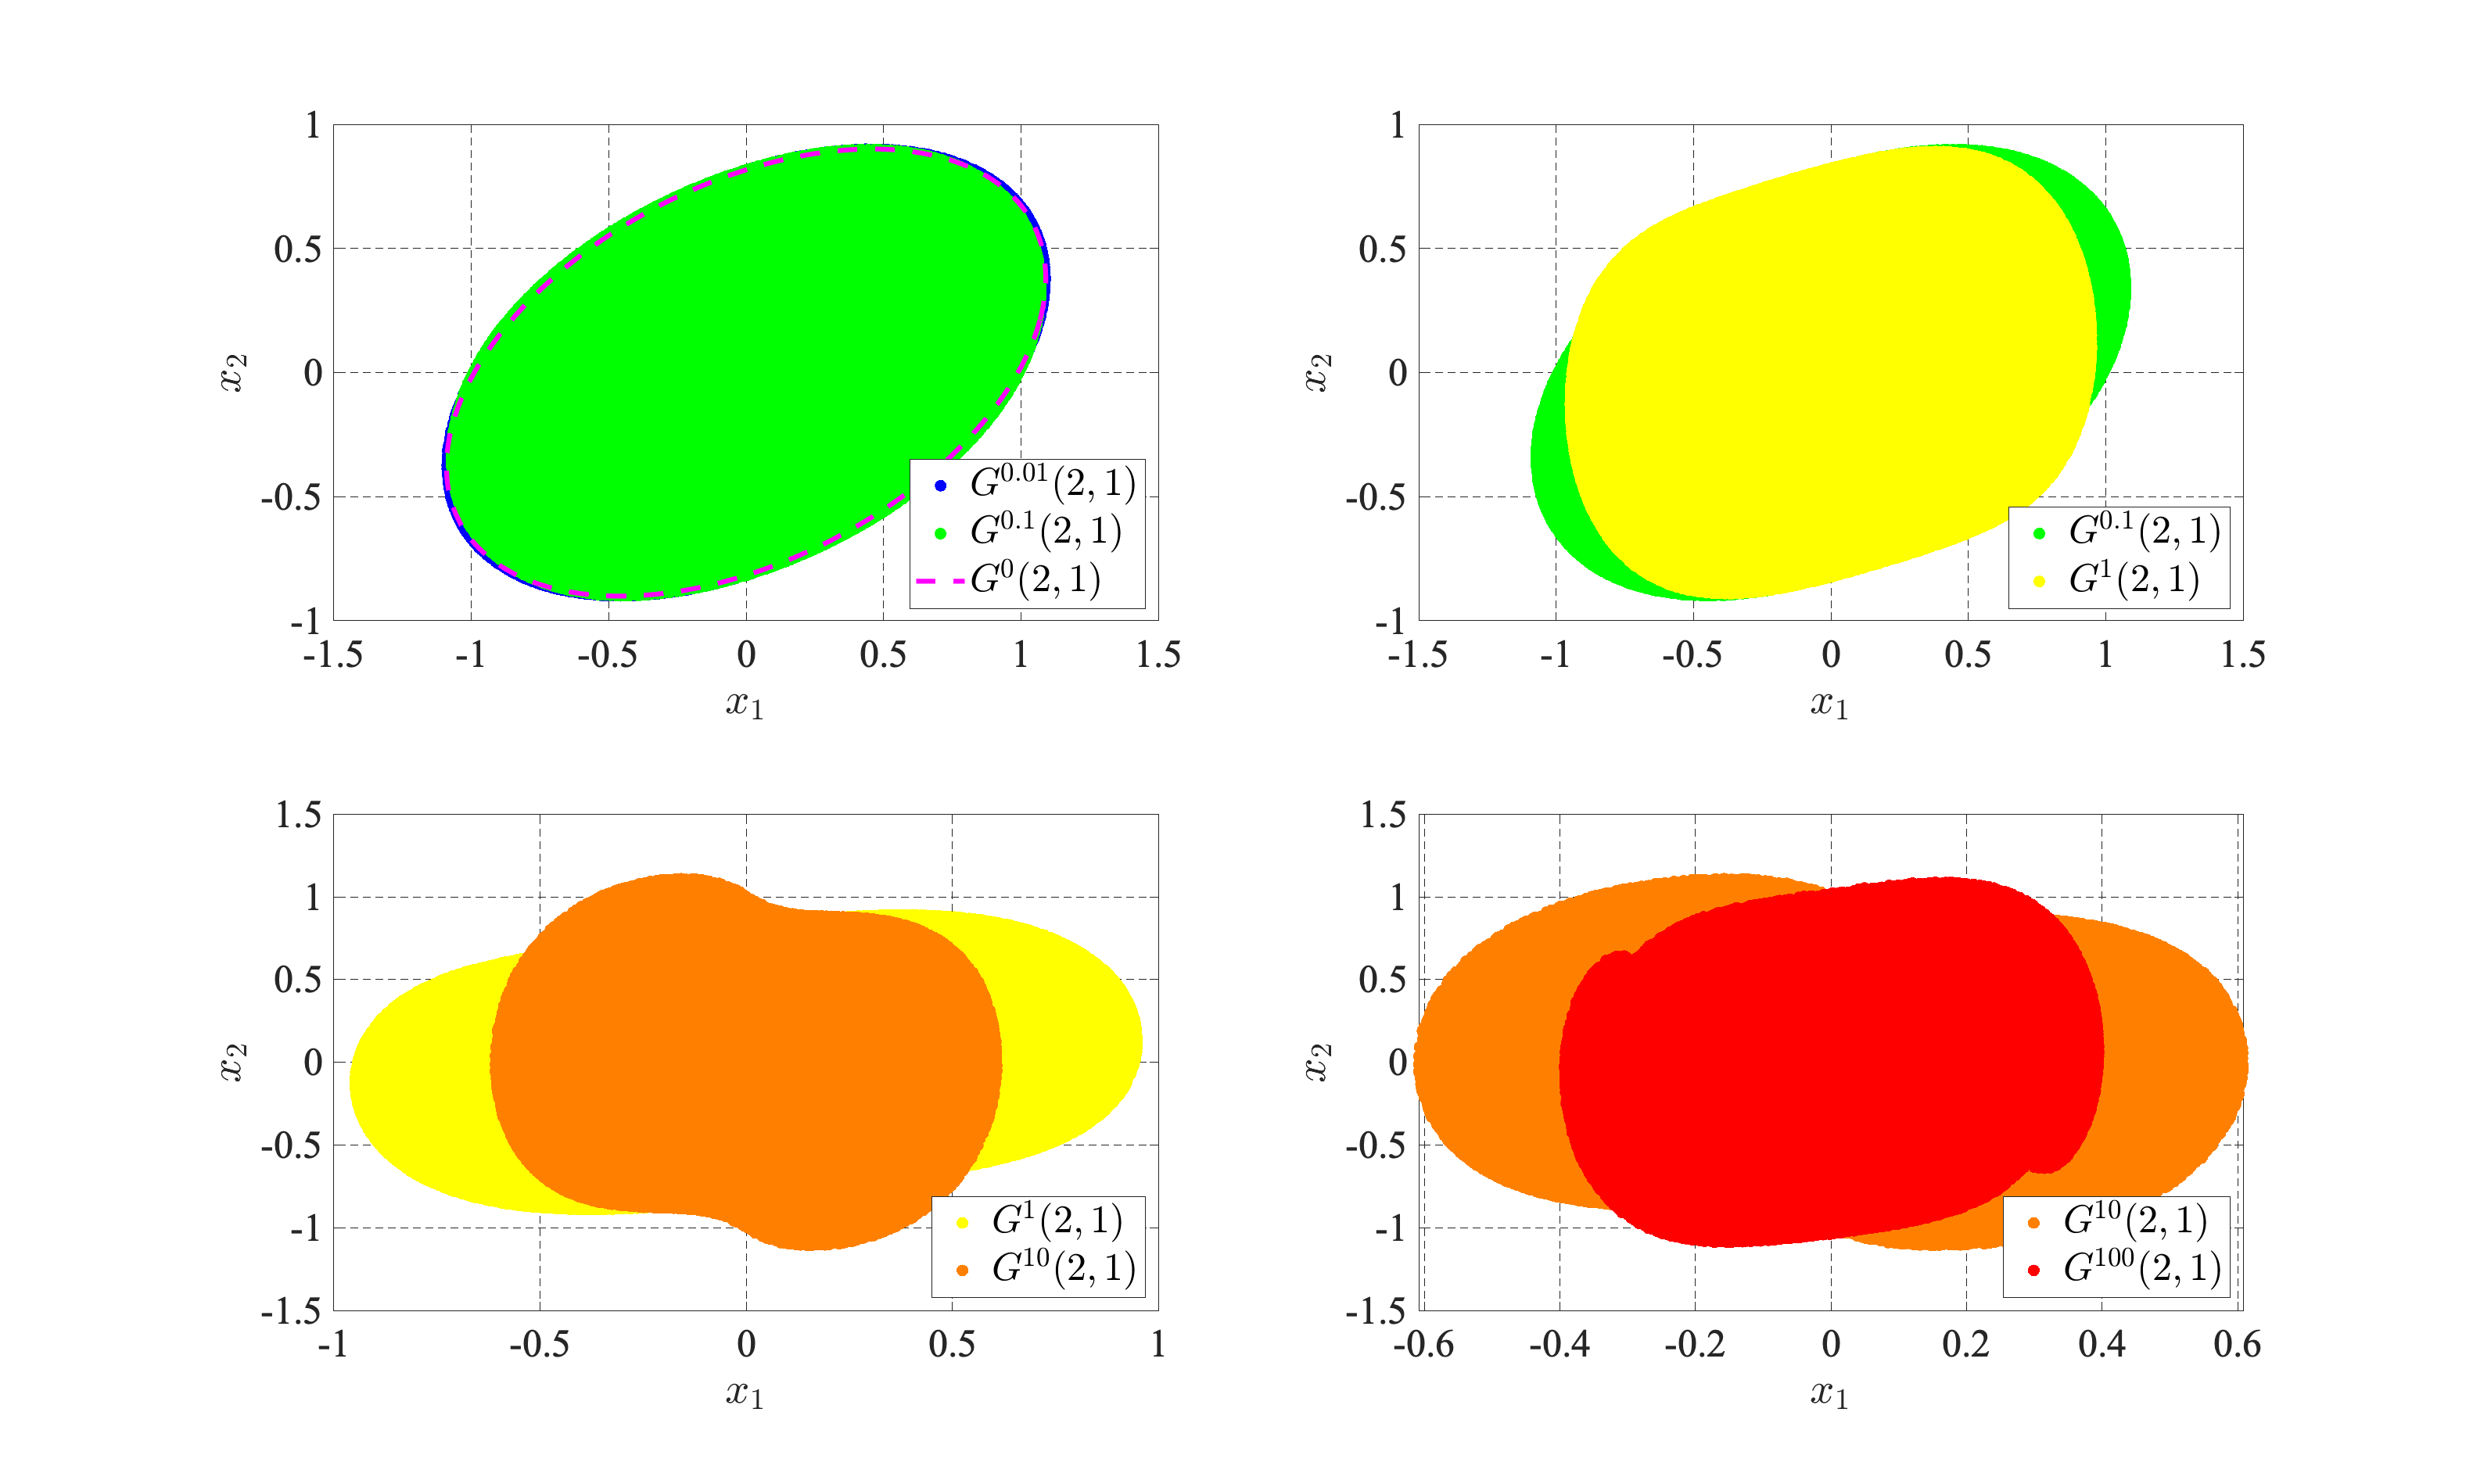
\includegraphics[width=\textwidth]{images/Osipov_QuaziDuffing.eps}}
		\caption{The reachable sets of Duffing oscillator.}
		\label{fig:Duffing}
	\end{figure}
	
	Therefore, the requirements of Theorem \ref{th:ReachableSetsConvexity} are met for system \eqref{Duffing}, and the corresponding reachable sets should be convex for small parameter values. This is evident in Figure \ref{fig:Duffing}, which demonstrates the constructed reachable sets $G^{\varepsilon}(T,\mu) $ using numerical Monte-Carlo based technique \cite{Patent,Zykov}.
	
	It can be seen that sets $G^{0.01}(1,1) $ and $G^{0.1}(1,1) $ are close to set $G^{0}(1,1) $ constructed for the linear system. One can also see that the sets become non-convex as the parameter $\varepsilon$ increases. 
	
\end{pr}  % Example (Пример)
\begin{figure}[ht]
	\centerline{
		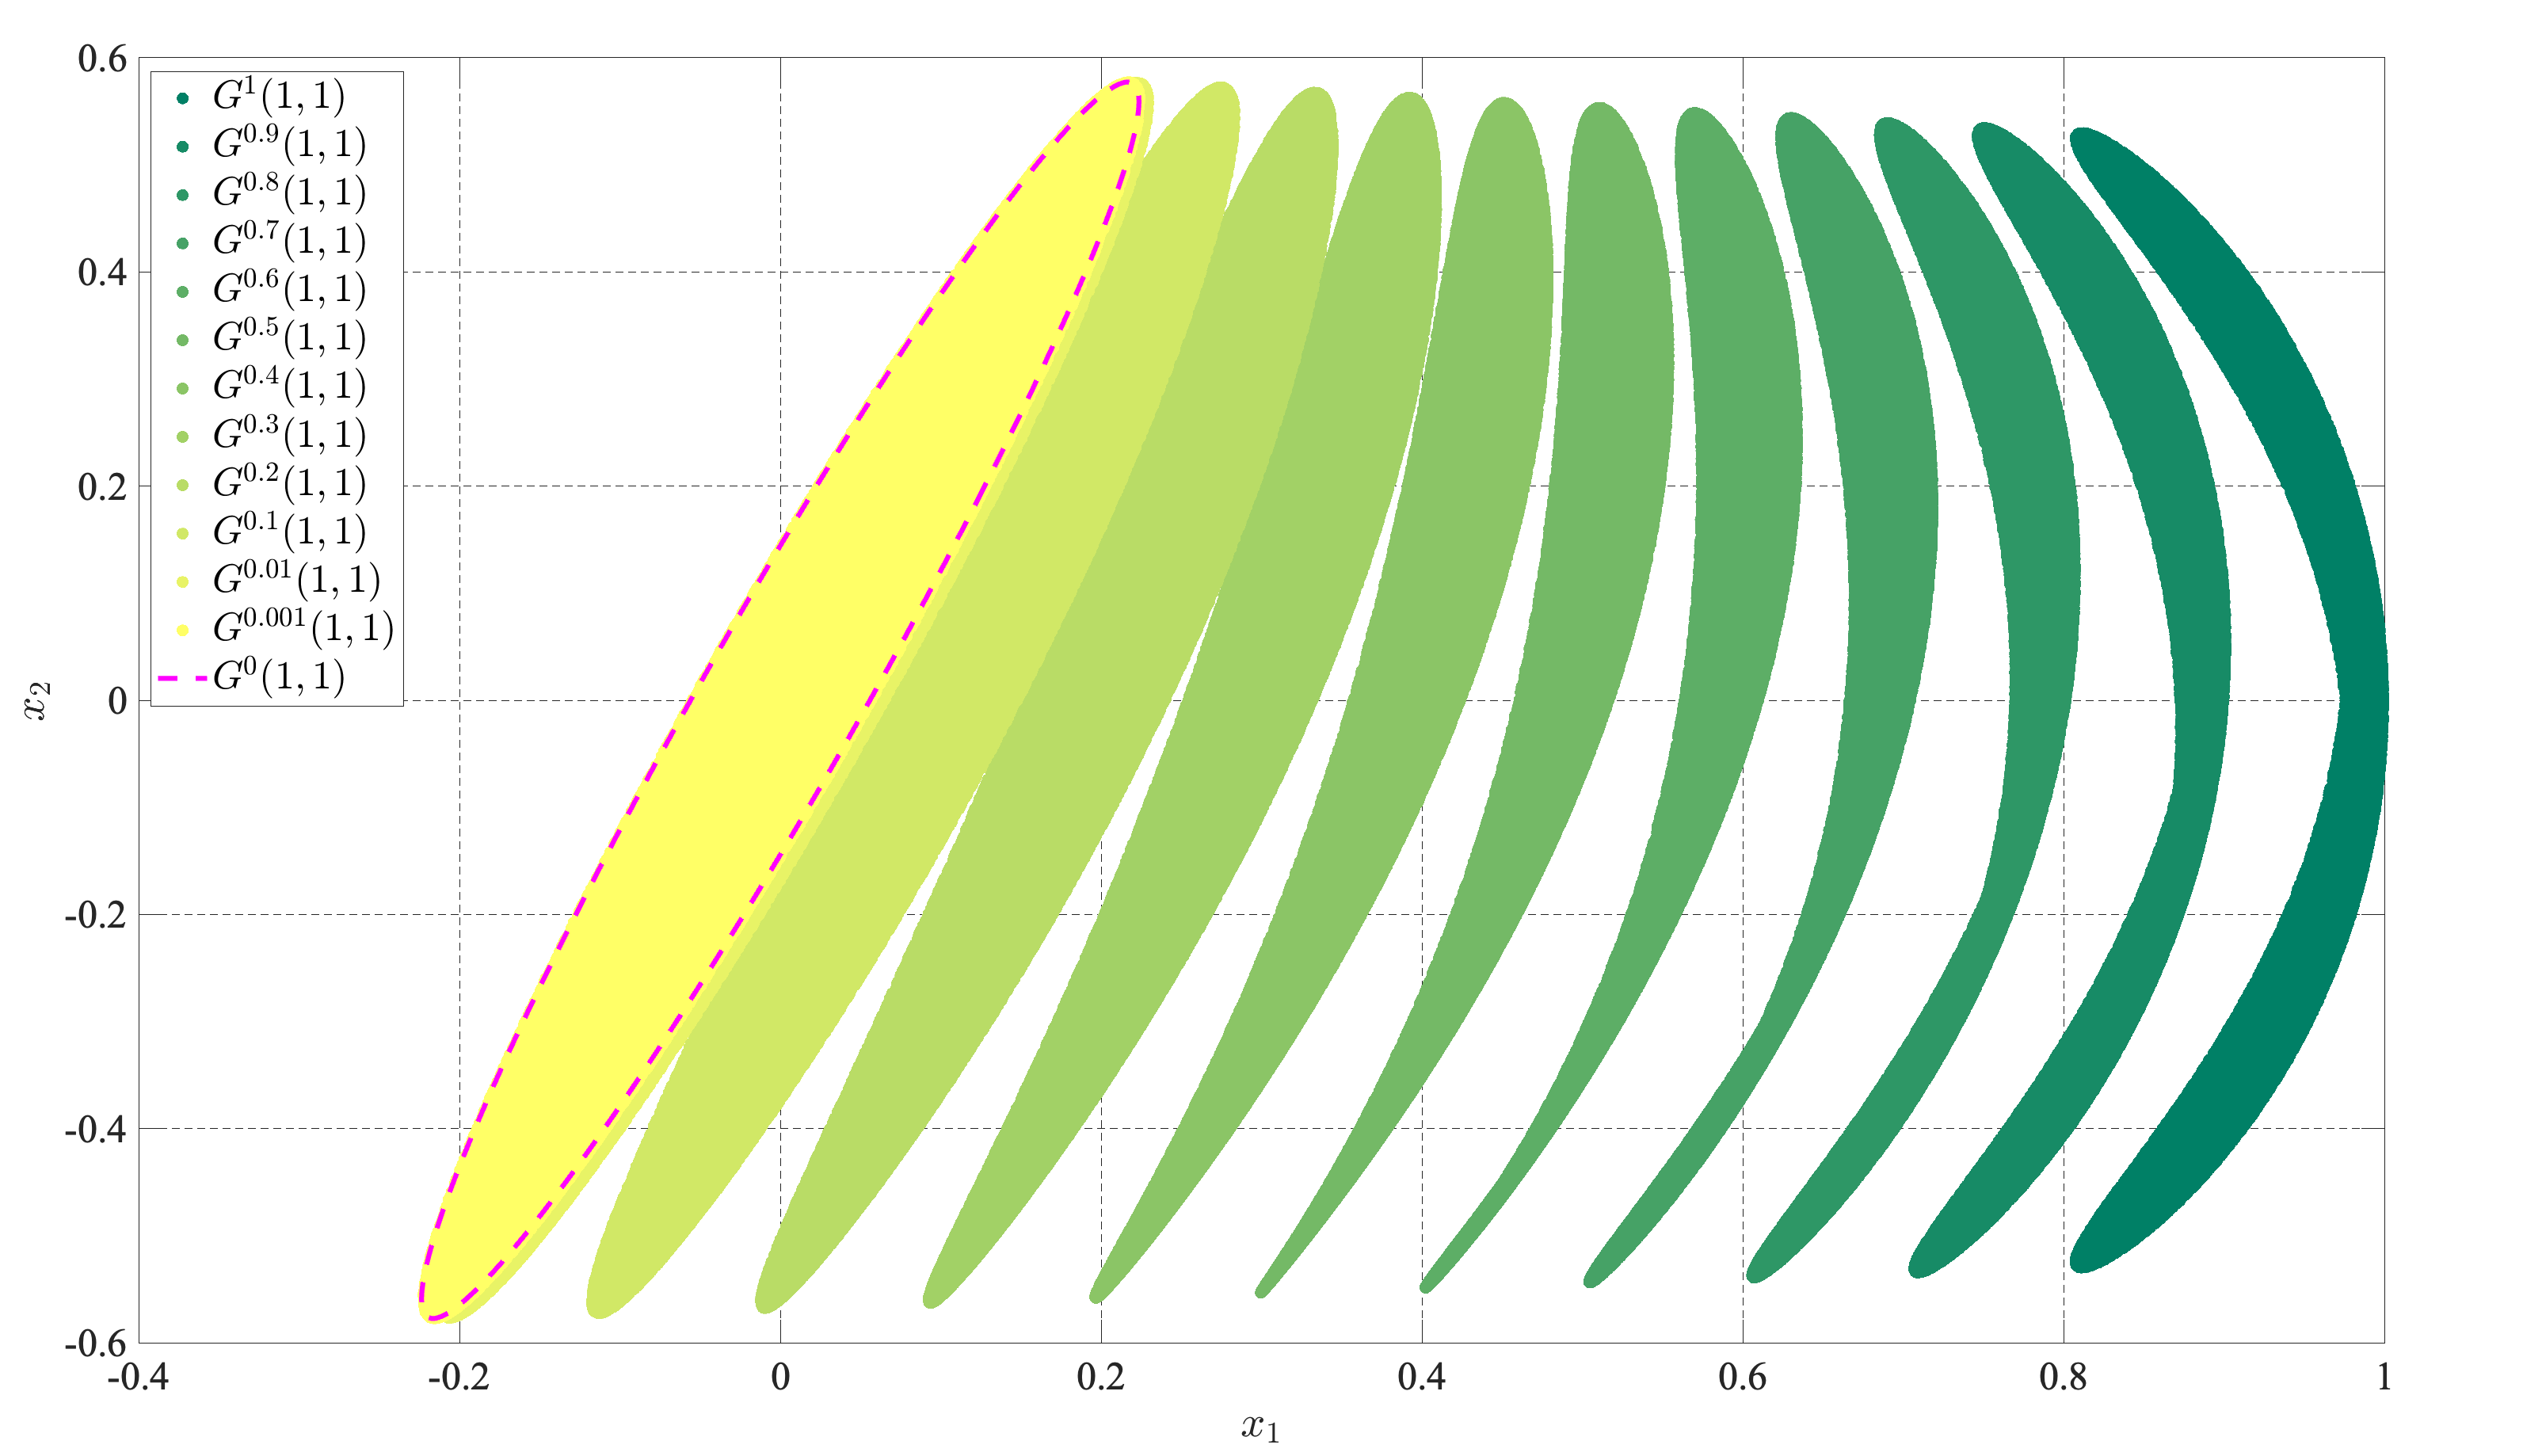
\includegraphics[width=\textwidth]{images/Osipov_QuaziDubins.eps}}
	\caption{The reachable sets of system \eqref{Linear+Dubins}.}
	\label{fig:LinearDubins}
\end{figure}
\begin{pr}  
	Second system under study is
	\begin{gather}\label{Linear+Dubins}
		\begin{pmatrix} 
			\dot{x}_1 \\
			\dot{x}_2 \\ 
			\dot{x}_3 \end{pmatrix} = 
		\begin{pmatrix}
			0 & 1 & 0 \\
			0 & 0 & 1 \\
			0 & 0 & 0
		\end{pmatrix}
		\begin{pmatrix} 
			x_1 \\
			x_2 \\ 
			x_3 \end{pmatrix} + 
		\varepsilon
		\begin{pmatrix}
			\cos x_3 - x_2\\
			\sin x_3 - x_3 \\
			0
		\end{pmatrix} + 
		\begin{pmatrix}
			0 \\ 0 \\ 1
		\end{pmatrix} u.
	\end{gather}
	When $\varepsilon = 0$, the equations \eqref{Linear+Dubins} describe a linear system with matrices 
	\begin{gather*}
		A = \begin{pmatrix} 0 & 1 & 0\\
			0 & 0 & 1\\ 
			0 & 0 & 1 
		\end{pmatrix}, \quad B = \begin{pmatrix}
			0\\
			0\\
			1
		\end{pmatrix},
	\end{gather*}
	and when $\varepsilon = 1$, they describe a unicycle. The nonlinear term comprises of a small parameter and the function
	\begin{gather*}
		f(x) = \begin{pmatrix}
			\cos x_3 - x_2\\
			\sin x_3 - x_3 \\
			0
		\end{pmatrix}.
	\end{gather*}
	
	The initial state is zero $x_1(0) = x_2(0) = x_3(0) $, the constraints on the controls are the same as in the first example, but we will consider this system on the time interval $0 \leqslant t \leqslant 1$.
	
	Similar to the previous example, the conditions of Assumption \ref{as:right_hand_side_conditions} are satisfied, allowing the application of Theorem \ref{th:ReachableSetsConvexity}. Figure \ref{fig:LinearDubins} displays the projections in the plane $(x_1,x_2)$ of the numerically constructed reachable sets $G^{\varepsilon}(T,\mu)$ for the system \eqref{Linear+Dubins}. 
	
	It can be seen that projections of sets $G^{0.001}(1,1) $ and $G^{0.01}(1,1) $ are close to projection of set $G^{0}(1,1) $ constructed for the linear system. One can also see that the projections of sets become non-convex as the parameter $\varepsilon$ increases. 
\end{pr}  % Example (Пример)



\end{document}